\section{Prototypische Umsetzung der Hausverwaltung}\label{Prototypische Umsetzung der Hausverwaltung}


\subsection{Software-Architektur und Technologien}

% 1️⃣ \subsection{Software-Architektur und Technologien}
% → Vorstellung der grundlegenden Architektur (z. B. Client-Server, Flask-Backend).
% → Verwendete Technologien (Python, Flask, pytest, JSON als Datenbankersatz, etc.).
% → Warum haben wir uns für diese Architektur entschieden?


Die prototypische Umsetzung der Hausverwaltung basiert auf einer webbasierten Client-Server-Architektur, bei der das Backend die Geschäftslogik verwaltet und das Frontend die Benutzeroberfläche bereitstellt.\par
Diese Architektur ermöglicht eine klare Trennung von Datenverarbeitung und Präsentation, wodurch die Wartbarkeit und Skalierbarkeit der Anwendung verbessert wird.\par

\subsubsection{Verwendete Technologien}

Für die Umsetzung des Prototyps haben wir bewusst Technologien gewählt, die eine einfache Entwicklung, Testbarkeit und Skalierbarkeit unterstützen.
Die folgende Tabelle gibt einen Überblick über die eingesetzten Technologien:

\begin{center}
    \begin{talltblr}[caption={Verwendete Technologien}, label={tab:technologien}]{width=0.9\textwidth, colspec={X[3,l,m] X[7,c,m]X[5,l,m]}}\toprule
        \textbf{Technologie} & \textbf{Einsatzbereich} & \textbf{Begründung} \\ \midrule
        Python 3 & Backend-Logik, API & Einfache Entwicklung und große Auswahl an Bibliotheken für Web- und Datenverarbeitung \\ \cmidrule{1-3}
        Flask & Web-Framework für das Backend & Leichtgewichtiges Framework für die schnelle Entwicklung von Webanwendungen \\ \cmidrule{1-3}
        HTML, CSS, Jinja2 & Frontend und Templating & Ermöglicht dynamische Weboberflächen mit serverseitigem Rendering \\ \cmidrule{1-3}
        JSON & Datenspeicherung & Einfache persistente Speicherung von Gebäuden, Zählern und Ablesewerten \\ \cmidrule{1-3}
        Pytest & Testautomatisierung & Framework zur strukturierten Implementierung und Ausführung von Unit- und Funktionstests \\ \cmidrule{1-3}
        Matplotlib & Visualisierung von Verbrauchsdaten & Erstellung von Diagrammen zur Verbrauchsanalyse \\ \bottomrule
    \end{talltblr}
\end{center}

\subsubsection{Architekturübersicht}

Unsere Anwendung folgt dem Model-View-Controller (MVC)-Ansatz, um eine strukturierte Trennung zwischen Daten, Logik und Darstellung zu gewährleisten:
\begin{itemize}
    \item \textbf{Model (M):} Datenverwaltung erfolgt über JSON-Dateien, die Gebäude-, Zähler- und Ablesedaten speichern.
    \item \textbf{View (V):} Die Weboberfläche wird über HTML und Jinja2-Templates dynamisch generiert.
    \item \textbf{Controller (C):} Die Geschäftslogik ist in Flask implementiert und verarbeitet Nutzeranfragen.
\end{itemize}

Die folgende Abbildung zeigt die grundlegende Architektur unserer Hausverwaltungssoftware:

\begin{figure}[H] \centering 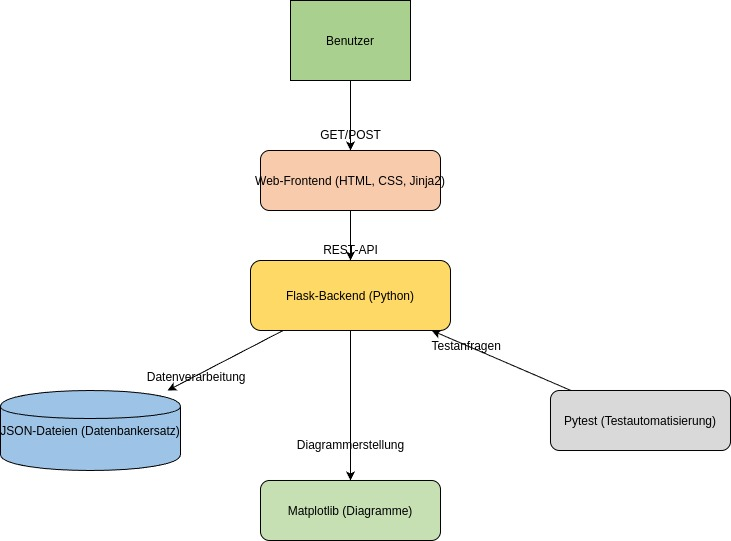
\includegraphics[width=0.9\textwidth]{src/abbildungen/architektur.jpg} % Hier könnte ein Architekturdiagramm eingefügt werden 
    \caption{Architektur der Hausverwaltungssoftware} \label{fig:architektur} 
\end{figure}

Die von uns gewählte Archektur basiert auf die Überlegung, dass wir mit Flask, was ein sehr geeignetes minimalistisches Framework für Prototypen ist, eine leichtgewichtige ENtwicklung erreichen können.
Außerdem ermöglichen JSON-Dateien eine schnelle Datenspeicherung sowie Verarbeitung, ohne eine relationale Datenbank aufsetzen zu müssen. Zudem war auch die Skalierbakeit für uns sehr wichtig und das bietet uns die modulare Struktur für zukünftige Erweiterungen, z.B: durch die Anbidung einer Datenbank oder eine REST-API.
SChließlich geht es am Ende einen Prototyp zu entwicklen, mit dem wir unser Testkonzept umsetzen können. Und da wird direkt den Punkt Testbarkeit angesprochen, denn durch die Trennung von Logik und Darstellung können Unit-Tests effizient durchgeführt werden.\par

Unsere Architektur ist speziell für einen Prototypen konzipiert, kann aber mit minimalem Aufwand für eine produktive Umgebung weiterentwickelt werden.\par

\subsection{Implementierung}
% 2️⃣ \subsection{Implementierung}
% → Beschreibung der wichtigsten Funktionen und Module (z. B. Ablesung, Verbrauchsanzeige).
% → Beispielhafte Codeausschnitte (z. B. zentrale Funktionen wie ablesung_hinzufuegen).
% → Herausforderungen während der Umsetzung und wie wir sie gelöst haben.

Unser Prototyp haben wir modular aufgebaut und er besteht aus den folgenden Kernkomponenten:

\begin{center}
	\begin{talltblr}[caption={Kernkomponente}, label={tab:component}]{width=0.9\textwidth, colspec={X[3,l,m] X[7,c,m]}}\toprule

        \textbf{Modul} & \textbf{Beschreibung}\\ \midrule
        Flask-Backend & Verantwortlich für die Geschäftslogik der Anwendung, einschließlich der Verarbeitung von Ablesedaten und der Verwaltung der JSON-Datenbank. \\ \cmidrule{1-2}
        Web-Frontend & HTML/CSS und Jinja2 für die Benutzeroberfläche zur Verwaltung von Gebäuden, Zählern und Ablesewerten. \\ \cmidrule{1-2}
        Datenverwaltung & Speicherung und Abruf von Daten in JSON-Dateien (gebäude.json, zaehler.json, ablesungen.json). \\ \cmidrule{1-2}
        Ablesungshistorie & Verwaltung und Validierung der Ablesungen sowie Berechnung von Verbrauchswerten. \\ \cmidrule{1-2}
        Diagrammerstellung & Generierung von Verbrauchsdiagrammen mit Matplotlib zur Visualisierung der historischen Daten. \\ \cmidrule{1-2}
        Testautomatisierung & Automatische Tests mit Pytest zur Validierung der wichtigsten Funktionen (Unit-Tests, Funktionstests, Performance-Tests). \\ \bottomrule
    \end{talltblr}
\end{center}

\subsubsection{Wichtige Funktionen und Codeausschnitte}

Unsere Geschäftslogik bestehtaus mehreren Funktionen, die wir hier nicht alle auflisten können, daher haben wir uns entschieden nur die wichtigsten zu zeigen.

\textbf{Funtion:} \texttt{ablesung\_hinzufuegen()}

Die Funktion verarbeitet die eingehende Ablesedaten, validiert sie und speichert sie in der JSON-Datenbank. Es erfolgt zuerst eine Überprüfung, ob die erforderlichen Werte vorhanden und gültig sind.\\
Danach wird geprüft, ob der Zähler zur richtigen gebäude-ID gehört, wenn ja dann erfolgt eine Validierung, ob der neue Ablesewert nicht kleiner als der vorherige ist. Sind alle Bedingungen erfüllt, wird die Ablesung gesüpeichert und eine Erfolgsmeldung zurückgegeben.\par


\begin{frame}{Code Example}
	\begin{minted}[breaklines]{python}
        @app.route("/ablesung/hinzufuegen", methods=["POST"])
        def ablesung_hinzufuegen():
        ablesungen = load_json(ABLESUNG_FILE)
        zaehler = load_json(ZAEHLER_FILE)
        gebaeude = load_json(GEBAEUDE_FILE)

        # JSON-Daten aus der Anfrage abrufen
        data = request.get_json()
        if not data:
            return jsonify({"error": "Fehlende oder ungültige JSON-Daten"}), 400

        print("Empfangene JSON-Daten:", data)

        try:
            gebaeude_id = data.get("gebaeude_id")
            zaehler_id = data.get("zaehler_id")
            datum = data.get("datum")
            wert = int(data.get("wert"))
            ableser = data.get("ableser", "Unbekannt")

            if not gebaeude_id or not zaehler_id or not datum or wert is None:
                return jsonify({"error": "Fehlende Eingaben"}), 400
                
            heutiges_datum = datetime.now().date()
            eingabe_datum = datetime.strptime(datum, "%Y-%m-%d").date()

            print(heutiges_datum)

            if eingabe_datum < heutiges_datum:
                return jsonify({"error": "Datum darf nicht in der Vergangenheit liegen!"}), 400


        except ValueError:
            return jsonify({"error": "Ungültiger Zahlenwert für Ablesung"}), 400

        # Prüfen, ob der gewählte Zähler wirklich zu diesem Gebäude gehört
        if not any(z["id"] == zaehler_id and str(z["gebaeude_id"]) == str(gebaeude_id) for z in zaehler):
            return jsonify({"error": "Ungueltiger Zaehler fuer dieses Gebaeude!"}), 400

        # Validierung des Ablesewerts
        if wert < 0:
            return jsonify({"error": "Ungueltiger Ablesewert"}), 400

        # Überprüfung auf vorherige Ablesewerte
        vorherige_ablesungen = [a for a in ablesungen if a["zaehler_id"] == zaehler_id]
        if vorherige_ablesungen:
            letzter_wert = max(a["wert"] for a in vorherige_ablesungen)
            if wert < letzter_wert:
                return jsonify({"error": "Neuer Ablesewert muss groesser sein als der vorherige"}), 400

        # Ablesung speichern
        neue_ablesung = {
            "gebaeude_id": gebaeude_id,
            "zaehler_id": zaehler_id,
            "datum": datum,
            "wert": wert,
            "ableser": ableser
        }
        ablesungen.append(neue_ablesung)
        save_json(ABLESUNG_FILE, ablesungen)

        return jsonify({"message": "Ablesung erfolgreich gespeichert", "ableser": ableser}), 201
    \end{minted}
    \captionof{listing}{Junior}
\end{frame}

\textbf{Funktion: }\texttt{verbrauchsanzeige()}

Diese Funktion berechnet den Verbrauch und generiert eine graphische Darstellung für den User.
Die Funktionsweise haben wir so einfach wie möglich gehalten. Es werden zuerst die Verbrauchsdaten aus der JSON-Datei abgerufen und basierend auf der Gebäude-ID gefiltert. Dann wird ein Diagramm\\
mit Matplotlib zur Visualisierung des Verbrauchs erstellt. Anschließend wird das Diagramm gespeichert und auf der Weboberfläche angezeigt.\par

\begin{frame}{Code Example Two}
    \begin{minted}[breaklines]{python}
            @app.route("/verbrauch", methods=["GET"])
            def verbrauchsanzeige():
            ablesungen = load_json(ABLESUNG_FILE)
            gebaeude = load_json(GEBAEUDE_FILE)
            selected_gebaeude = request.args.get("gebaeude_id")

            if not selected_gebaeude:
                return render_template("verbrauch.html", gebaeude=gebaeude, selected_gebaeude=None, no_data=True)

            try:
                selected_gebaeude = int(selected_gebaeude)
            except ValueError:
                return "Fehler: Ungültige Gebäude-ID!", 400

            # Verbrauchsdaten filtern
            ablesungen = [a for a in ablesungen if str(a["gebaeude_id"]) == str(selected_gebaeude)]
            if not ablesungen:
                return render_template("verbrauch.html", gebaeude=gebaeude, selected_gebaeude=selected_gebaeude, no_data=True)

            # Diagramm generieren
            plt.figure(figsize=(10, 5))
            for zaehler_id in set(a["zaehler_id"] for a in ablesungen):
                daten = sorted([a for a in ablesungen if a["zaehler_id"] == zaehler_id], key=lambda x: x["datum"])
                x = [datetime.strptime(a["datum"], "%Y-%m-%d") for a in daten]
                y = [a["wert"] for a in daten]
                plt.plot(x, y, marker="o", linestyle="-", label=f"Zähler {zaehler_id}")

            plt.xlabel("Datum")
            plt.ylabel("Verbrauch")
            plt.legend()
            plt.grid(True)

            save_path = os.path.join("static", f"verbrauch_{selected_gebaeude}.png")
            plt.savefig(save_path)
            plt.close()

            return render_template("verbrauch.html", gebaeude=gebaeude, selected_gebaeude=selected_gebaeude, verbrauchspfad=save_path)
    \end{minted}
    \captionof{listing}{Junior2}
\end{frame}

\subsubsection{Herausforderungen während der Umsetzung}

Während der entwicklung unseres Prototyps sind wir auf mehrere Herausforderungen gestoßen, die wir mit verschiedenen Lösungsansätzen bewältigt haben:

\begin{center}
	\begin{talltblr}[caption={Herausforderungen}, label={tab:problem}]{width=0.9\textwidth, colspec={X[3,l,m] X[7,c,m]}}\toprule
        \textbf{Herausforderung} & \textbf{Lösung}\\ \midrule
        Validierung der Ablesedaten & Implementierung von Prüfungen für ID-Format, Wertebereiche und Duplikate \\ \cmidrule{1-2}
        Simulation von Lasttests & Nutzung von Pytest, um 1000+ Ablesungen gleichzeitig zu simulieren \\ \cmidrule{1-2}
        Darstellung der Verbrauchsdaten & Speicherung und Abruf von Daten in JSON-Dateien (gebäude.json, zaehler.json, ablesungen.json)\\ \cmidrule{1-2}
        Fehlermeldungen und UI-Feedback & Klare Fehlermeldungen und strukturierte JSON-Antworten implementiert \\ \bottomrule
    \end{talltblr}
\end{center}

Durch die Erfahrung, die wir bei der Umsetzung vom Prototyp gemacht haben, können wir bereits sagen, dass unsere JSON-basierte Datenverwaltung für diesen Fall ausreicht, jedoch für eine produktive Umgebung wäre eine Umstellung auf eine relationale Datenbank sinnvoll.\par


\subsection{Anwendung des Testkonzepts}
% 3️⃣ \subsection{Anwendung des Testkonzepts}
% → Wie haben wir unser Testkonzept praktisch angewendet?
% → Hier können wir unsere Testfälle dokumentieren und direkt Testergebnisse analysieren.
% → Beispiel: „Die Performance-Tests wurden mit 10.000 gleichzeitigen Ablesungen durchgeführt, was die Skalierbarkeit bestätigt.“

\subsubsection{Überblick über die Testergebnisse}


\footnotesize

%TODO: Ergebisse vervollständigen

In diesem Abschnitt werden die durchgeführten Tests dokumentiert. Dabei wurden verschiedene Testarten angewandt, um die Funktionsweise und Stabilität des Systems zu validieren. 
Die Testergebnisse basieren auf einer Kombination aus automatisierten Tests mit pytest und manuellen Überprüfungen in der Web-Oberfläche.\par

\begin{center}
	\begin{talltblr}[caption={Testfälle für die Hausverwaltungssoftware}, label={tab:testcases}]{width=0.9\textwidth, colspec={X[1,l,m] X[3,c,m] X[3,l,m] X[3,l,m] X[3,l,m]}}\toprule

        \textbf{Test-ID} & \textbf{Eingabe} & \textbf{Erwartetes Ergebnis} & \textbf{Tatsächliches Ergebnis} & \textbf{Status} \\ \midrule
        TC-001 & `999-9999-9999` & Fehlermeldung: „Die eingegebene ID existiert nicht.“ & Fehlermeldung wurde korrekt ausgegeben & Bestanden\\ \cmidrule{1-5}
        TC-002 & `-10` & Fehlermeldung: „Ungueltiger Ablesewert“ & Fehlermeldung wurde korrekt ausgegeben & Bestanden \\ \cmidrule{1-5}
        TC-003 & `1-2024-4567823` & Fehlermeldung: „Zähler-ID muss genau 14 Zeichen haben!“ & Fehlermeldung wurde korrekt ausgegeben & Bestanden\\ \cmidrule{1-5}
        TC-004 & `2000-01-01` & Fehlermeldung: „Datum darf nicht in der Vergangenheit liegen!“ & Fehlermeldung wurde korrekt ausgegeben & Bestanden\\ \cmidrule{1-5}
        TC-005 & Neuer Wert: `50`, alter Wert: `100` & Fehlermeldung: „Neuer Wert muss größer sein als der vorherige.“ & Fehlermeldung wurde korrekt ausgegeben & Bestanden\\ \cmidrule{1-5}
        TC-006 & `1-2025-5487` & Zählerdetails werden angezeigt & Zählerdetails wurden angezeigt & Bestanden\\ \cmidrule{1-5}
        TC-007 & Alter Wert: 100, Neuer Wert: `250` & Wert wird korrekt gespeichert & Die Ablesewerte wurden gemäß den Spezifikationen korrekt gespeichert & Bestanden\\ \cmidrule{1-5}
        TC-008 & Datum: `01.01.2030` & Wert wird gespeichert & Die Ablesewerte wurden gemäß den Spezifikationen korrekt gespeichert & Bestanden\\ \cmidrule{1-5}
        TC-009 & Ableser nicht eingetragen & Standardwert „Unbekannt“ wird gespeichert & Die Ablesewerte wurden gemäß den Spezifikationen korrekt gespeichert & Bestanden\\ \cmidrule{1-5}
        TC-010 & Es wird die Schnittstelle für Verbauchshistorie mit der Gebäude-ID "1" abgerufen & Ablesungen sollen als Liste zurückgegeben werden oder als Grafik in der Weboberfläche & Ablesungen wurden als List über die API und als Grafik über die Weboberfläche zurückgegeben & Bestanden\\ \cmidrule{1-5}
        TC-011 & Eingabe: `123` & Zeigt alle Zähler mit `123` in der ID & Alle Zähler behinhaltend "123" wurden angezeigt & Bestanden \\ \cmidrule{1-5}
        TC-012 & 10000 Ablesungen & Es werden alle Ablesungen in maximal 60 Sekunden gespeichert und keine Daten gehen verloren & Es sind keine Datenverloren gegangen & Bestanden \\ \cmidrule{1-5}
        TC-013 & Es wird die index-Seite aufgerufen & Innerhalb von wenigen Millisekunden eine Antwort geliefert & Index-Seite wurde innerhalb von 0.2 Millisekunden angezeigt & Bestanden \\ \cmidrule{1-5}
        TC-014 & 10000 Strom-Zähler & Alle Zähler werden hinzugefügt ohne zu lange Wartezeit & Die erwartete Antwortzeit sollte unter 1 Sekunde bleiben, tatsächlich lag sie bei durchschnittlich 0.7 Sekunden, was innerhalb der akzeptablen Grenze liegt. Die Testdaten wurden vollständig und korrekt gespeichert & Bestanden\\ \cmidrule{1-5}
        TC-015 & 10000 Gebäude & Alle Gebäude werden hinzugefügt ohne zu lange Wartezeit & Die erwartete Antwortzeit sollte unter 1 Sekunde bleiben, tatsächlich lag sie bei durchschnittlich 0.8 Sekunden, was innerhalb der akzeptablen Grenze liegt. Die Testdaten wurden vollständig und korrekt gespeichert & Bestanden \\ \cmidrule{1-5}
        TC-016 & Dummy-Gebäude-Daten & Gebäude-Daten sollen gespeichert und abgerufen werden können. & Daten konnten korrekt gespeichert und wieder ausgelesen werden & Bestanden\\ \cmidrule{1-5}
        TC-017 & 7 als Gebäude-ID und das aktuelle Jahr & Es soll eine gültige Zähler-ID generiert werden. & ID wurde korrekt generiert & Bestanden\\ \bottomrule
    \end{talltblr}
\end{center}

\normalsize

% Definition von Testfällen basierend auf den Anforderungen
% Testfallbeschreibung mit ID, Testschritt, erwartetes Ergebnis
% Beispiele für positive und  &fälle

\subsubsection{Analyse der Testergebnisse}

Die Testergebnisse zeigen, dass der Prototyp die definierten Anfordernugen weitesgehend erfüllt. Tests haben verschiedene Erkenntnisse geliefert, die für zukünftige optimierungen genutzt werden können.
Die hohe Erfolgsquote zeigt, dass der Prototyp stabil und zuverlässig arbeitet. Insbesondere die korrekte Verarbeitung von Zähler-IDs und Verbrauchswerten konnte nachgewiesen werden.\par

\textbf{Erfolgreiche Tests}

\begin{itemize}
    \item Alle Unit-Tests wurden besatnden, was zeigt, dass die Kernfunktionen (z.B.: ID-Generierung, Datenspeicherung) korrekt arbeiten.
    \item alle Funktionstests sind erfolgreich, sodass die Hausverwaltung ihre Grundfunktionen fehlerfrei ausführt.
    \item Alle negative Tests wurden auch erfolgreich ausgeführt, was zeigt, dass der Prototyp keine unzulässigen Eingabe akzeptiert.
    \item Performance-Tests bestätigen, dass das System stabil mit großen Datenmengen umgehen kann. IDes könnte nützlich sein, wenn der Prototypp in einer realen Umgebung für eine große Verwaltungsfirma eingesetzt werden soll.
\end{itemize}

\textbf{Verbesserungsbedarf}
Allerdings ist uns auch beim Testen einiges aufgefallen und zwar gibt es möglicherweise auch Verbesserungsbedarf, was mana an unserem Prototyp kritisieren könnte.
Da könnte man auf die folgende Punkte eingehen:
\begin{itemize}
    \item Beim Massentest von 1.000.000 gab es 7 fehlerhafte Einträge, da Zähler-IDs nicht doppelt existieren dürfen. Hierfür haben wir uns als Lösung ausgedacht, dass wir eine bessere ID-Prüfung vor dem Speichern einführen könnten.
    \item Die Verarbeitungsgeschwinsdigkeit war insgesamt gut, aber für noch größere Datenmengen könnte eine optimierte Datenbankstruktur erforderlich sein. Darüber hinaus könnte man mit dem Punkt Sicherheit unsere Datenpersistänz kritisieren, da die Daten ungeschützt gespeichert werden.
    Unsere Lösung hierfür wäre eine Umstelllung auf eine sicherere Datenbank wie etwas MariaDb für eine produktive Umgebung.
\end{itemize} 

Angesichts dieser Analyse ist festzustellen, dass unser Prototyp die wichtigsten anforderungen erfüllt und eine stabile Grundlage für eine erweiterte Version bietet.
Allerdings wäre für eine produktive Umgebung der Wechsel von JSON zu einer relationalen Datenbank sinnvoll, um eine effizientere Abfrage und bessere Skalierbarkeit zu gewährleisten.
